\part{Calcolo Differensiale}

\chapter{Calcolo Differensiale}

\section{Preliminari}
La base canonica di $R^n$ è indicata con $(e_1,...,e_i)$, $e_i$ è il vettore di $R^n$ con tutte le componenti nulle tranne la i-esima che vale 1.\\
Un generico vettore $x$ si può quindi scrivere come combinazione lineare dei vettori di base $x=\sum\limits_{j=1}^{i}\alpha_j e_j$.\\
Nel caso n=2 è usata la notazione $(x,y)=xi+yj$\\
Nel caso n=3 è usata la notazione $(x,y,z)=xi+yj+zk$\\
Alcune classi di funzioni $f:A\subseteq\R^n\rightarrow\R^m$ hanno nomi particolari:
\begin{itemize}
	\item 
	$n=1$,$m=1$:$f$ è una funzione reale di una variabile reale;
	\item 
	$n=1$,$m>1$:$f$ è una curva in $R^m$ (purché sia almento continua e definita su un intervallo)
	\item 
	$n>1$,$m=1$:$f$ è un campo scalare
	\item
	$n>1$,$m>1$:$f$ è un campo vettoriale
\end{itemize}
\section{Derivate Pardiali e Direzionali}
\definition
sia $f:A\subseteq\R^2\rightarrow\R$ e $(x_0,y_0)\in\AA$, $h,k\in\R$
chiamo derivata parziale rispetto a $x$ di $f$ in $(x_0,y_0)$ la quantità (se esiste finita)
$$\partial_xf(x_0,y_0) = \lim\limits_{h\rightarrow{0}}\frac{f(x_0+h,y_0)-f(x_0,y_0)}{h}$$
chiamo derivata parziale rispetto a $y$ di $f$ in $(x_0,y_0)$ la quantità (se esiste finita)
$$\partial_yf(x_0,y_0) = \lim\limits_{h\rightarrow{0}}\frac{f(x_0,y_0+k)-f(x_0,y_0)}{h}$$
\definition
sia $f:A\subseteq\R^n\rightarrow\R^m$ e $x_0\in\AA$, $i=1,...,n$
$$\partial_if(x_0) = \lim\limits_{t\rightarrow{0}}\frac{f(x_0+te_i)-f(x_0)}{t}$$
dove $(e_1,...,e_n)$ rappresentano la base canonica di $R^n$\\
\observation nella prima definizione la derivata è un valore reale mentre nella seconda è un vettore di $R^m$\\
\observation le proprietà e le regole di derivazione sono le stesse di Analisi 1
\definition
sia $f:A\subseteq\R^2\rightarrow\R$ e $(x_0,y_0)\in\AA$, sia $v\in\R^2 con \left\| v\right\|=1 $
ciamo derivata nella direzione $v$ della funzione $f$ nel punto $(x_0,y_0)$ il limite (se esiste finito)\\
$$D_vf(x_0,y_0) = \lim\limits_{t\rightarrow{0}}\frac{f(x_0+tv_1,y_0+tv_2)-f(x_0,y_0)}{t}$$
dove $v_1,v_2$ sono le componenti di $v(v=\begin{bmatrix}v_1\\v_2\end{bmatrix})$
\definition
sia $f:A\subseteq\R^n\rightarrow\R^m$ e $x_0\in\AA$, sia $v\in\R^n con \left\| v\right\|=1 $
ciamo derivata nella direzione $v$ della funzione $f$ nel punto $x_0$ il limite (se esiste finito)\\
$$D_vf(x_0) = \lim\limits_{t\rightarrow{0}}\frac{f(x_0+tv)-f(x_0)}{t}$$
\proposition
(ANALISI 1): sia $f:A\subseteq \R\rightarrow\R$ e $x_0\in\AA$\\
$f$ è differenziabile $\Leftrightarrow$ $\exists m\in \R $ t.c. $f(x_0+h)=f(x_0)+mh+o(h)$ per $h\rightarrow 0$
...\\
...\\
...\\

\section{Derivata Totale}
\definition
sia $f:A\subseteq \R^n\rightarrow \R^m$ e $x_0\in\AA$ \\
$f$ è differenziabile in $x_0\rightleftharpoons$ $\exists M\in Mat(mxn) : f(x_0+h) = f(x_0)+Mh+o(h)$ per $h\rightarrow 0$ 
\definition
siano $f,g : A\subseteq \R^n\rightarrow \R^m$ e $x_0$ di accumulazione per A \\
$f=o(g)$ per $x\rightarrow x_0 \rightleftharpoons \lim\limits_{x->x_0}\frac{\left\| f(x)\right\| }{\left\| g(x)\right\| }$
\definition
sia $f:A\subseteq \R^2\rightarrow \R$ e $(x_0,y_0)\in\AA$ \\
$f$ è differenziabile in $(x_0,y_0)\rightleftharpoons$ $f(x_0+h,y_0+k) = f(x_0)+m_1h+m_2k+o(\sqrt{h^2+k^2})$ per $(h,k)\rightarrow (0,0)$
\definition
siano $f,g : :A\subseteq \R^2\rightarrow \R$ e $(x_0,y_0)$ di accumulazione per $A$ \\
$f=o(g)$ per $(x,y)\rightarrow (x_0,y_0) \rightleftharpoons \lim\limits_{(x,y)->(x_0,y_0)}\frac{\left\| f(x,y)\right\| }{\left\| g(x,y)\right\| }$
\proposition{(Unicità della derivata totale)}
sia $f:A\subseteq \R^n\rightarrow \R^m$, $x_0\in\AA$, $M_1$,$M_2\in Mat(mxn)$\\
$M1$ derivata totale di $f$ in $x_0$,\\
$M2$ derivata totale di $f$ in $x_0$,\\
allora $M1=M2$\\
\begin{proof}
	poiche $M_1$ e $M_2$ sono derivate totali di $f$ nel punto $x_0$,\\
	$f(x_0+h) = f(x_0)+M_1h+o(h)$ per $h\rightarrow 0$\\
	$f(x_0+h) = f(x_0)+M_2h+o(h)$ per $h\rightarrow 0$\\
	facendo la differenza membro a membro delle precedenti ottengo che $(M_1-M_2)h=o(h)$ per $h\rightarrow 0$\\
	Scelto $h=te_i$, dove $e_i$ è un vettore della base canonica, si ottiene $(M_1-M_2)te_i=o(h)$ quindi\\
	$\lim\limits_{t\rightarrow 0}\frac{(M_1-M_2)te_i}{t\left\| e_i\right\| } = \lim\limits_{t\rightarrow 0}(M_1-M_2)e_i = 0$, poiché $e_i$ è un vettore non nullo deve essere $(M_1-M_2)=0$ quindi $M_1 = M_2$\\
\end{proof}
\observation
L'ultima riga della dimostrazione dice che le applicazioni lineari $M_1$ e $M_2$ hanno le stesse immagini sui vettori della base canonica, quindi coincidono.

\proposition
sia $f:A\subseteq \R^n\rightarrow \R^m$, $x_0\in\AA$\\
$f$ è differenziabile in $x_0$ $\Rightarrow$ $f$ è continua in $x_0$\\
DIMOSTRAZIONE\\

..\\
..\\
..\\
..\\
..\\
..\\


\theorem{Differenziale Totale}
sia $f:A\subseteq \R^n\rightarrow \R^m$ e $x_0\in\AA$.\\
$\exists \partial_{i}f(x)\;\forall i=1,...,n definite \forall x$ in un intorno di $x_0$\\
$\partial{i}f$ è continua in $x_0$\\
$\Rightarrow f$ è differenziabile in $x_0$\\

\theorem{Differenziale Totale}
sia $f:A\subseteq \R^2\rightarrow \R$ e $(x_0,y_0)\in\AA$.\\
$\exists \partial_{x}f(x,y)$ e $\exists \partial_{y}f(x,y)$ definite $\forall x$ in un intorno di $(x_0,y_0)$\\
$\partial_{x}f(x,y)$ e $\exists \partial_{y}f(x,y)$ continue in $x_0$\\
$\Rightarrow f$ è differenziabile in $(x_0,y_0)$\\
\begin{proof}
	devo dimostrare che
	$$\lim\limits_{(h,k)\rightarrow (0,0)}\frac{f(x_0+h,y_0+k)-f(x_0,y_0)-\nabla f(x_0,y_0\begin{bmatrix}h\\k\end{bmatrix})}{\sqrt{h^2+k^2}} = 0$$
	dove $\nabla f(x_0,y_0)= \begin{bmatrix}\partial_xf(x_0,y,0) && \partial_yf(x_0,y_0)\end{bmatrix}$\\

	\begin{tikzpicture}
	\pgfmathsetmacro\MAX{8}
	\pgfmathsetmacro\XZ{\MAX / 3 }
	\pgfmathsetmacro\YZ{\MAX / 3 }
	\pgfmathsetmacro\XZh{\MAX / 3 *2}
	\pgfmathsetmacro\YZk{\MAX / 3 *2}
	\coordinate (X0Y0) at (\XZ,\YZ);
	\coordinate (X0hY0) at (\XZh,\YZ);
	\coordinate (X0Y0k) at (\XZ,\YZk);
	\coordinate (X0hY0k) at (\XZh,\YZk);
	
	\draw[->] (0,0) -- (\MAX,0) node[anchor=north west] {x};
	\draw[->] (0,0) -- (0,\MAX) node[anchor=south east] {y};
	\draw[dotted] (\XZ,0) -- (\XZ,\MAX);
	\draw[dotted] (0,\YZ) -- (\MAX,\YZ);
	\draw[dotted] (\XZh,0) -- (\XZh,\MAX);
	\draw[dotted] (0,\YZk) -- (\MAX,\YZk);
	\draw node[anchor=north] at (\XZ,0) {$x_0$};
	\draw node[anchor=north] at (\XZh,0) {$x_0+h$};
	\draw node[anchor=east] at (0,\YZ) {$y_0$};
	\draw node[anchor=east] at (0,\YZk) {$y_0+k$};
	\draw node at (X0Y0) {$\bullet$};
	\draw node at (X0Y0k) {$\bullet$};
	\draw node at (X0hY0) {$\bullet$};
	\draw node at (X0hY0k) {$\bullet$};
	\draw node[anchor=north east] at (X0Y0) {$(x_0,y_0)$};
	\draw node[anchor=south east] at (X0Y0k) {$(x_0,y_0+k)$};
	\draw node[anchor=north west] at (X0hY0) {$(x_0+h,y_0)$};
	\draw node[anchor=south west] at (X0hY0k) {$(x_0+h,y_0+k)$};
	
	\draw[<-] (\XZ,\MAX*4/10) -- (\XZ,\MAX*6/10);
	\draw[<-] (\XZh,\MAX*4/10) -- (\XZh,\MAX*6/10);
	\draw[<-] (\MAX*4/10,\YZ) -- (\MAX*6/10,\YZ);
	\draw[<-] (\MAX*4/10,\YZk) -- (\MAX*6/10,\YZk);
	
	\draw node at (\XZ,\MAX/2) {A};
	\draw node at (\XZh,\MAX/2) {B};
	\draw node at (\MAX/2,\YZ) {C};
	\draw node at (\MAX/2,\YZk) {D};
	\end{tikzpicture}
	devo calcolare lo scarto della funzione tra i punti $(x_0+h,y_0+k)$ e $(x_0,y_0)$. Ho a disposizione le derivate parziali che mi danno informazioni lungo le parallele agli assi quindi non muovo lungo la diagonale ma lungo i percorsi D,A e B,C\\
	Il limite  (<-) fa zero se il numeratore è zero, allora guardo solo quello.\\
	$$f(x_0+h,y_0+k) -f(x_0,y_0)- \partial{x}f(x_0,y_0)h - \partial{y}f(x_0,y_0)k$$
	riscrivo tale quantità seguendo il percorso D,A
	$$ [f(x_0+h,y_0+k) - f(x_0+h,y_0)] + [f(x_0+h,y_0) - f(x_0,y_0)] - \partial{x}f(x_0,y_0)h - \partial{y}f(x_0,y_0)k$$
	chiamo $\varphi (x) = f(x,y_0)$ quindi $f(x_0+h,y_0)-f(x_0,y_0) = \varphi (x_0+h)-\varphi (x_0)$\\
	la funzione $\varphi $ è una funzione reale di una variabile reale ed in virtù del teorema di Lagrange $\varphi (x_0+h)-\varphi (x_0) = \varphi^{'}(x_0 + \beta h)h$ per $\beta\in ]0,1[ $, per come definita $\varphi$ si ha che $\varphi^{'}(x_0 + \beta h)h = \partial_{x}f(x_0+\beta h,y_0)h$\\
	con un rangionamento del tutto analogo si può definire $\varPsi (x) = f(x_0+h,y)$ e si ha che $\varPsi (y_0+h)-\varPsi (y_0) = \varPsi^{'}(y_0 + \alpha k)k = \partial_{y}f(x_0+h,y_0+\alpha k)k$ per $\alpha\in ]0,1[ $\\
	Quindi
	$$ [f(x_0+h,y_0+k) - f(x_0+h,y_0)] + [f(x_0+h,y_0) - f(x_0,y_0)] - \partial{x}f(x_0,y_0)h - \partial{y}f(x_0,y_0)k = $$
	$$= [\partial_{x}f(x_0+\beta h,y_0)h] + [\partial_{y}f(x_0+h,y_0+\alpha k)k] - \partial{x}f(x_0,y_0)h - \partial{y}f(x_0,y_0)k = $$
	$$= [\partial_{x}f(x_0+\beta h,y_0)h - \partial{x}f(x_0,y_0)h] + [\partial_{y}f(x_0+h,y_0+\alpha k)k  - \partial{y}f(x_0,y_0)k] $$
	Adesso la riscrivo recuperando il denominatore 	'e devo verificare che il limite per $(h,k)\rightarrow (0,0)$ tenda a zero.\\
	
	$$[\partial_{x}f(x_0+\beta h,y_0)-\partial{x}f(x_0,y_0)] \frac{h}{\sqrt{h^2+k^2}} + [\partial_{y}f(x_0+h,y_0+\alpha k) - \partial{y}f(x_0,y_0)]\frac{k}{\sqrt{h^2+k^2}} $$
	Le derivate parziali sono continue quindi per $(h,k)\rightarrow (0,0)$ i numeratori tendono a zero\\
	Inoltre le due franzioni per $(h,k)\rightarrow (0,0)$ sono quantità limitate tra $-1$ e $1$ quindi si può dire che il limite cercato fa 0.
\end{proof}


\section{Regole di Derivazione}
\proposition
Siano $f,g: A\subseteq \R^n \rightarrow \R^m$ e $x_0\in\AA$\\
$f$ differenziabile in $x_0$, $g$ differenziabile in $x_0$ allora $f+g$ differenziabile in $x_0$ e $D(f+g)(x_0) = Df(x_0)+Dg(x_0)$
\begin{proof}
	$f$ è differenziabile, allora $f(x_0+h)=f(x_0)+Df(x_0)h+o(h)$ per $h\rightarrow 0$\\
	anche $g$ lo è, quindi $g(x_0+h)=g(x_0)+Dg(x_0)h+o(h)$ per $h\rightarrow 0$\\
	sommando membro a membro si ottiene  $(f+g)(x_0+h)=(f+g)(x_0)+[Df(x_0)+Dg(x_0)]h+o(h)$ per $h\rightarrow 0$\\
	Questa è la definizione di differenziabilità, allora $f+g$ è differenziable e $D(f+g)(x_0) = Df(x_0)+Dg(x_0)$
\end{proof}

\proposition
Sia $f: A\subseteq \R^n \rightarrow \R^m$ e $x_0\in\AA$ e $\lambda\in \R$\\
$f$ differenziabile in $x_0$ allora $\lambda f$ differenziabile in $x_0$ e $D(\lambda f)(x_0) = \lambda Df(x_0)$
\begin{proof}
	$f$ è differenziabile, allora $f(x_0+h)=f(x_0)+Df(x_0)h+o(h)$ per $h\rightarrow 0$\\
	valuto ora $(\lambda f)(x_0+h)=(\lambda f)(x_0)+\lambda Df(x_0)h+o(h)$ per $h\rightarrow 0$\\
	Questa è la definizione di differenziabilità, allora $\lambda f$ è differenziable e $D(\lambda f)(x_0) = \lambda Df(x_0)$
\end{proof}

\proposition
Sia $g: A\subseteq \R^n \rightarrow \R^m$ e $x_0\in\overset{\circ}{A}$\\
Sia $f: B\subseteq \R^m \rightarrow \R^p$ e $g(x_0)\in\overset{\circ}{B}$\\
$f$ differenziabile in $g(x_0)$, $g$ differenziabile in $x_0$ allora $f\circ g$ differenziabile in $x_0$ e $D(f\circ g)(x_0) = Df(g(x_0))*Dg(x_0)$
\begin{proof}
	$g$ è differenziabile in $x_0$, allora $g(x_0+h)=f(x_0)+Dg(x_0)h+o(h)$ per $h\rightarrow 0$\\
	$f$ è differenziabile in $g(x_0)$ allora $g(g(x_0)+k)=f(g(x_0))+Df(g(x_0))k+o(k)$ per $k\rightarrow 0$\\
	valuto ora 
	$$(f\circ g)(x_0+h) = f(g(x_0+h)+Dg(x_0)h+o(h)) = $$ 
	$$=f(g(x_0))+Df(g(x_0))(Dg(x_0)h+o(h))+o(Dg(x_0)h+o(h)) = $$
	$$=(f\circ g)(x_0) + Df(g(x_0))Dg(x_0)h+Df(g(x_0))o(h)+Dg(x_0)o(h)+o(h)$$
	
	con $h$ un vettore $n\times 1$\\
	con $Dg$ una matrice $m\times n$\\
	con $Df$ una matrice $p\times m$\\
	
	da rivedere un pochino ....
	
	Questa è la definizione di differenziabilità, allora $f\circ g$ è differenziable e $D(f\circ g)(x_0) = Df(g(x_0))Dg(x_0)$
\end{proof}
\proposition DERIVATA DEL PRODOTTO

\section{La Formula degli Accrescimenti Finiti}
\definition
Siano $x_0,x_1\in \R^n$, si dice segmento di estremi $x_0$ e $x_1$ l'insieme $S={tx_1+(1-t)x_0 : t\in[0,1]}$
\proposition{Formula degli accrescimenti finiti}\\
Sia $f:A\subseteq \R^n\rightarrow \R^m$, $x_0,x_1\in\overset{\circ}{A}$, $S$ il segmento di estremi $x_0,x_1$, sia $f\in C^1(A,\R^m)$ allora $\left\| f(x_1)-f(x_0) \right\|\le \sup\limits_{x\in S}\left\|Df(x)\right\|\left\|x_1-x_0\right\|$
\observation
$\left\| A \right\|$ con $A\in Mat(n\times m)$,  $\left\| A \right\|=\sup\limits_{\left\| x \right\|=1: x\in \R^n}\left\| Ax \right\| = \sup\limits_{x\in \R^n \textbackslash \{0\}}\frac{\left\| Ax \right\| }{\left\| x \right\| } $ questa è chiamata norma operativa\\
NOTA:\\
$$\left\| Ax \right\| \le \left\| A \right\| \left\| x \right\|  $$
$$\left\| AB \right\| \le \left\| A \right\| \left\| B \right\|  $$
\begin{proof}
	sia $F:[0,1]\rightarrow \R$ che $t\rightarrow f(tx_1+(1-t)x_0)$\\
	%moltiplicando per $v\in \R^m$ ottengo una funzione in $\R^m$\\
	La funzione $F$ è una funzione reale di variabile reale , posso quindi applicare il teorema di Lagrange $F(1)-F(0)=F^{'}(\theta)1$ quindi $f(x_1)-f(x_0) = Df(\theta x_1 + (1-\theta)x_0)(x_1-x_0)$\\
	scelto $v\in \R^m$ con $v = \frac{f(x_1)-f(x_0)}{\left\| f(x_1)-f(x_0)\right\| }$ moltiplico entrambi i membri per $v$ si ottiene $v(f(x_1)-f(x_0)) = vDf(\theta x_1 + (1-\theta)x_0)(x_1-x_0)$\\
	... da finire per bene
\end{proof}
\definition
Sia $C\in \R^n$, $C$ è convesso $\rightleftharpoons$ $\forall x_0,x_1\in C$ anche $S_(x_0,x_1) = \{tx_1+(1-t)x_0 : t\in[0,1]\}\subseteq C$ù

\proposition
sia $f:A\subseteq \R^n \rightarrow \R^m$, $A$ è aperto connesso e $f\in C^1(A;\R^m)$ e $Df=0$ allora $f$ è costante su $A$\\
..... disegnino e bozza di dimostrazione

\proposition
sia $f:A\subseteq \R^n \rightarrow \R^m$, $A$ è aperto convesso e $f\in C^1(A;\R^m)$ e $Df=0$ allora $f$ è costante su $A$\\
..... disegnino e bozza di dimostrazione

\proposition
sia $f:A\subseteq \R^n \rightarrow \R^m$, $A$ è aperto connesso e $f\in C^1(A;\R^m)$ e $Df=0$ allora $f$ è costante su $A$\\
..... disegnino e bozza di dimostrazione

\observation vale anche sugli insiemi connessi poiche in questi posso congiungere due qulunque punti con una poligonale interamente contenuta nell'insieme e con i lati paralleli agli assi. Attraverso la formula degli accrescimenti finiti posso calcolare la $f$ nei due estremi passando per tutti gli spigoli della poligonale.(Uno spigolo è un segmento quindi si puòapplicare il teorema precedente)\\

si po dire qulcosa sulle funzioni lineari tipo c1, lips ....\\

\section{Derivate Seconde}
Sia $f:A\subseteq \R^n \rightarrow \R^m$ sappiamo che $Df(x_0)\in Mat(m\times n)$, allora $Df:A\subseteq \R^{n} \rightarrow \R^{m\times n}$ cie\'e la derivata è una funzione a valori in $Mat(m\times n)$, ne segue che $D(D(F)):A\subseteq \R^n \rightarrow \R^{m\times n\times n}$
\definition
sia $f:A\subseteq \R^n \rightarrow \R^m$ derivabile parzialmente in $x_0$ lungo $e_i$. Se la funzione $\frac{\partial{f}}{\partial{x_i}}$ è derivabile parzialmente lungo $e_j$ in $x_0$, la quantità $\frac{\partial}{\partial{x_j}}\frac{\partial{f}}{\partial{x_i}}(x_0)$ è la derivata seconda di $f$ in $x_0$ rispetto $x_i,x_j$ e si indica $\frac{\partial^2f}{\partial{x_j}\partial{x_i}}(x_0)$
\definition
sia $f:A\subseteq \R^n \rightarrow \R^m$ e $x_0\in\AA$\\
$f$ differenziabile due volte in $xo \rightleftharpoons f$ è differenziabile in un intorno di $x_0$ e $f$ è differenziabile in $x_0$
\observation
con la notazione della definizione precedente, $f$ è una funzione definita in un intorno di $x_0$ con valori in $Mat(m\times n)$, spazio identificabile con $R^{m\times n}$
\observation
per una funzione scalare $f:A\subseteq \R^n \rightarrow \R$, la derivara prima è un vettore (il gradiente $\nabla$ in $R^{1\times n}$), la derivata seconda è una matrice in $R^{1\times n \times n}$, la derivata terza è una super matrice ...
\definition
sia $f:A\subseteq \R^n \rightarrow \R$ e $x_0\in\AA$, $f$ ammette tutte le derivate parziali seconde in $x_0$. La matrice di queste derivate seconde si chaiama Matrice Hessiana di $f$ in $x_0$
$$H_f(x_0)=D^2f(x_0) = \begin{bmatrix}
\frac{\partial^2f}{\partial{x_1}\partial{x_1}} && \frac{\partial^2f}{\partial{x_2}\partial{x_1}} && \dotsb && \frac{\partial^2f}{\partial{x_n}\partial{x_1}} \\
\frac{\partial^2f}{\partial{x_1}\partial{x_2}} && \frac{\partial^2f}{\partial{x_2}\partial{x_2}} && \dotsb && \frac{\partial^2f}{\partial{x_n}\partial{x_2}} \\
\vdots && \vdots && \ddots && \vdots \\
\frac{\partial^2f}{\partial{x_1}\partial{x_n}} && \frac{\partial^2f}{\partial{x_2}\partial{x_n}} && \dotsb && \frac{\partial^2f}{\partial{x_n}\partial{x_n}} \\
\end{bmatrix}$$ 
ESEMPI:\\
...\\
...\\
...\\

\section{Il Lemma di Schwarz}
\proposition
sia $f:A\subseteq \R^n\rightarrow \R^m$ e $x_0\in \AA$. Fino ...\\
$\exists \partial^2_{ij}f(x)$ e $\exists \partial^2_{ji}f(x)$ in un intorno di $x_0$ e continue in $x_0 \Rightarrow$ ....\\

CASO n=2 m=1
\proposition
sia $f:A\subseteq \R^2\rightarrow \R^1$ e $(x_0,y_0)\in \AA$. .....\\
$\exists \partial^2_{xy}f(x,y)$ e $\exists \partial^2_{yx}f(x,y)$ in un intorno di $(x_0,Y_0)$ e continue in $(x_0,y_0) \Rightarrow$ ....\\
\begin{proof}
	prendo una quantità $q=f(x_0+h,y_0+k)-f(x_0+h,y_0)-f(x_0,y_0+k)+f(x_0,y_0)$\\
	\begin{tikzpicture}
	\pgfmathsetmacro\MAX{8}
	\pgfmathsetmacro\XZ{\MAX / 3 }
	\pgfmathsetmacro\YZ{\MAX / 3 }
	\pgfmathsetmacro\XZh{\MAX / 3 *2}
	\pgfmathsetmacro\YZk{\MAX / 3 *2}
	\coordinate (X0Y0) at (\XZ,\YZ);
	\coordinate (X0hY0) at (\XZh,\YZ);
	\coordinate (X0Y0k) at (\XZ,\YZk);
	\coordinate (X0hY0k) at (\XZh,\YZk);
	
	\draw[->] (0,0) -- (\MAX,0) node[anchor=north west] {x};
	\draw[->] (0,0) -- (0,\MAX) node[anchor=south east] {y};
	\draw[dotted] (\XZ,0) -- (\XZ,\MAX);
	\draw[dotted] (0,\YZ) -- (\MAX,\YZ);
	\draw[dotted] (\XZh,0) -- (\XZh,\MAX);
	\draw[dotted] (0,\YZk) -- (\MAX,\YZk);
	\draw node[anchor=north] at (\XZ,0) {$x_0$};
	\draw node[anchor=north] at (\XZh,0) {$x_0+h$};
	\draw node[anchor=east] at (0,\YZ) {$y_0$};
	\draw node[anchor=east] at (0,\YZk) {$y_0+k$};
	\draw node at (X0Y0) {$\bullet$};
	\draw node at (X0Y0k) {$\bullet$};
	\draw node at (X0hY0) {$\bullet$};
	\draw node at (X0hY0k) {$\bullet$};
	
	%\draw node[anchor=north east] at (X0Y0) {$(x_0,y_0)$};
	%\draw node[anchor=south east] at (X0Y0k) {$(x_0,y_0+k)$};
	%\draw node[anchor=north west] at (X0hY0) {$(x_0+h,y_0)$};
	%\draw node[anchor=south west] at (X0hY0k) {$(x_0+h,y_0+k)$};
	\end{tikzpicture}\\
	L'idea è quella di calcolare $q$ in due modi diversi e osservare che le due scritture rappresentano la stessa quntità quindi sono uguali.\\
	$$q=[f(x_0+h,y_0+k)-f(x_0+h,y_0)]-[f(x_0,y_0+k)-f(x_0,y_0)]$$
	scelgo una funzione $\varphi(h)=f(x_0+h,y_0+k)-f(x_0+h,y_0)$
	$$q=\varphi(h)-\varphi(0) = \varphi^{'}(\alpha^{'} h)h$$
	valida per $\alpha^{'}\in ]0,1[$ e $\varphi^{'}(h)=\partial_{x}f(x_0+h,y_0+k)-\partial_{x}f(x_0+h,y_0)$
	$$q = [\partial_{x}f(x_0+\alpha^{'}h,y_0+k)-\partial_{x}f(x_0\alpha^{'}h+,y_0)]h$$
	scelgo una funzione $\varPhi(k)=\partial{x}f(x_0+h,y_0+k)$
	$$q=[\varPhi(k)-\varPhi(0)]h=\varPhi^{'}(\beta^{'}k)hk$$
	valida per $\beta^{'}\in ]0,1[$ e $\varPhi^{'}(k)=\partial_{y}\partial_{x}f(x_0+\alpha^{'}h,y_0+k)$
	$$q = \partial^2_{xy}f(x_0+\alpha^{'}h,y_0+\beta^{'}k)hk$$
	Ma $q$ può anche essere calcolata in un secondo modo
	$$q=[f(x_0+h,y_0+k)-f(x_0,y_0+k)]-[f(x_0+h,y_0)-f(x_0,y_0)]$$
	scelgo una funzione $\psi(k)=f(x_0+h,y_0+k)-f(x_0,y_0+k)$
	$$q=\psi(k)-\varphi(0) = \psi^{'}(\alpha^{''}k)k$$
	valida per $\alpha^{''}\in ]0,1[$ e $\psi^{'}(k)=\partial_{y}f(x_0+h,y_0+k)-\partial_{y}f(x_0,y_0+k)$
	$$q = [\partial_{y}f(x_0+h,y_0+\alpha^{''}k)-\partial_{y}f(x_0,y_0+\alpha^{''}k)]k$$
	scelgo una funzione $\Psi(h)=\partial{y}f(x_0+h,y_0+\alpha^{''}k)$
	$$q=[\Psi(h)-\varPhi(0)]k=\Psi^{'}(\beta^{''}k)hk$$
	valida per $\beta^{''}\in ]0,1[$ e $\Psi^{'}(h)=\partial_{x}\partial_{y}f(x_0+h,y_0+\beta^{''}k)$
	$$q = \partial^2_{xy}f(x_0+\alpha^{''}h,y_0+\beta^{''}k)hk$$
	Abbiamo quindi trovato che 
	$$ \partial^2_{xy}f(x_0+\alpha^{'}h,y_0+\beta^{'}k)hk = \partial^2_{xy}f(x_0+\alpha^{''}h,y_0+\beta^{''}k)hk$$
	Ci sarebbe un disegno ...\\
	...\\
	Abbiamo trovato che le derivate parziali seconde miste coincidono in due punti ad esempio quelli segnati con il cerchio, poiché $\alpha^{'},\alpha^{''},\beta{'},\beta^{''}$ li abbiamo scelti in $]0,1[$\\
	poiché $h,k$ li abbiamo scelti del tutto arbitrari allora facciamo il limite e poiché le due quantità sono uguali allora sono uguali anche i limiti.\\
	allora per $(h,k)\rightarrow (0,0)$ anche $\alpha^{'},\alpha^{''},\beta{'},\beta^{''}$ cambiano ma essendo limitati tra $]0,1[$ moltiplicandoli oer una quantità che tende a zero fa tutto zero.\\
	Usando la continuità, per $(h,k)\rightarrow (0,0)$ ottengo $\partial^2_{xy}f(x_0,y_0)=\partial^2_{yx}f(x_0,y_0)$
\end{proof}
\observation
$f:A\subseteq \R^n\rightarrow \R$\\
$Df(x_0)=\nabla f(x_0) \in Mat(1\times n)$\\
$H_f(x_0)\in Mat(n\times n)$\\
Il lemma di Schwarz dice che sotto opportune ipotesi la $H_f(x_0)$ è una matrice simmetrica, in questo caso non dobbiamo calcolare $n\times n$ termini, ma solo $\frac{n(n+1)}{2}$

\section{Sviluppo in Serie di Taylor al II Ordine}
sacbnijldasbndfcbuhsadebuhjdewsafbnmweasdbuijeasdhl...\\
sdadsadsfsdasdfasdfasdfafewrgvregrgbreqeragerwawfer...\\

\section{Il Teorema della funzione Implicita}
\definition
sia $X\in \R^n$ e $Y\in \R^m$, $f:X\times Y\to \mathbb\R^l$, $x_0\in \overset{\circ}{X}$, $y_0\in \overset{\circ}{Y}$.\\
L'equazone $f(x,y)=0$ definisce implicitamente una funzione $y=\varphi(x)$ in un intorno di $(x_0,y_0) \rightleftharpoons$
\begin{enumerate}
	\item $f(x_0,y_0)=0$, rappresenta un punto di partenza 
	\item $\exists \mathcal{X}$ intorno di $x_0$ e $\exists \mathcal{Y}$ intorno di $y_0$, in questo modo due intorno uno per punto, uno è l'insieme di partenza, l'altro l'insieme di arrivo
	\item $\exists\varphi:\mathcal{X}\rightarrow\mathcal{Y}$ t.c.: $f(x,y)=0$ con $x\in\mathcal{X}$ e $y\in\mathcal{Y} \Leftrightarrow y=\varphi(x)$
\end{enumerate}
ESEMPIO:\\
$m=n=l=1$, $f(x,y)=x^2+y^2+1$, questa equazione non definisce mai una funzione implicita poiche non è mai nulla\\
\\
ESEMPIO:\\
$m=n=l=1$, $f(x,y)=x^2+y^2-1$\\
	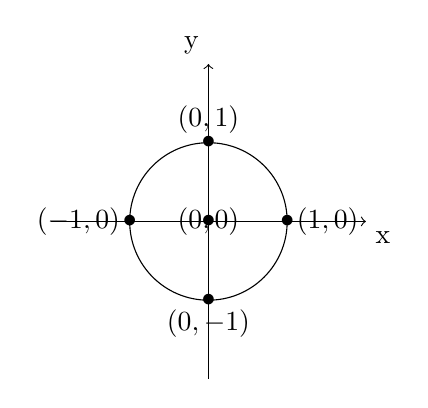
\begin{tikzpicture}
	\pgfmathsetmacro\MAX{2}
	\draw[->] (-\MAX,0) -- (\MAX,0) node[anchor=north west] {x};
	\draw[->] (0,-\MAX) -- (0,\MAX) node[anchor=south east] {y};
	\draw node at (0,0) {$(0,0)$};
	\draw node at (0,0) {$\bullet$};
	\draw node at (0,1) {$\bullet$};
	\draw node at (0,1) [anchor=south]{$(0,1)$};
	\draw node at (1,0) {$\bullet$};
	\draw node at (1,0) [anchor=west] {$(1,0)$};
	\draw node at (-1,0) {$\bullet$};
	\draw node at (-1,0) [anchor=east] {$(-1,0)$};
	\draw node at (0,-1) {$\bullet$};
	\draw node at (0,-1) [anchor=north]{$(0,-1)$};
	\draw (0,0) circle (1);
	\end{tikzpicture}\\
	Per prima cosa osservo che s possono trovare dei punti che rendono vera $f(x,y)=x^2+y^2-1=0$ e sono tutti i punti della circonferenza di centro l'origine degli assi e raggio unitario.\\
	il punto $(x_0,y_0)=(0,1)$ definisce implicitamente una funzione $y=\varphi(x)=\sqrt{1-x^2}$ con $\mathcal{X}=[-1,1]$ e $\mathcal{Y}=[0,1]$\\
	un primo problema è dovuto alla scelta degli intervalli $\mathcal{X},\mathcal{Y}$, per esempio posso scegliere $\mathcal{X}=[-\frac{1}{2},\frac{1}{2}]$ e $\mathcal{Y}=R^+$\\
	un secondo problema è la scelta del punto $(x_0,y_0)$, potrei scegliere il punto $(\frac{1}{\sqrt{2}},\frac{1}{\sqrt{2}})$\\
\observation
La stessa definizione può essere riscritta con la $x$ funzione della $y$ poiché a priori non c'è distinzione tra le variabili.
\proposition (caso lineare)\\
sia $f:R^n\times \R^m\rightarrow \R^p$ che $(x,y)\rightarrow Ax+By-C$ con $A\in Mat(p \times n), B\in (p \times m), B\in (p \times 1)$. Se $p=m$ cie\'e $B$ è un matrice quadrata, e $det(B)\ne 0$ cie\'e invertibile, allora\\
$\exists !\varphi : \R^n\rightarrow \R^m$ t.c.: $f(x,y)=0 \Leftrightarrow y=\varphi(x)$
\begin{proof}
	$f(x,y)=0\Leftrightarrow Ax+By=-C\Leftrightarrow By=-Ax+C\Leftrightarrow y=-B^{-1}Ax+B^{-1}C = \varphi(x)$
\end{proof}
\proposition
Sia $f:X\times Y\rightarrow \R^m$ con $X\in \R^n, Y\in \R^m$\\
Preso un punto $(x_0,y_0)$ con $x_0\in \overset{\circ}{X}$,$y_0\in \overset{\circ}{Y}$\\
se:
\begin{enumerate}
	\item $f$ continua in $X\times Y$
	\item $f(x_0,y_0)=0$
	\item $f$ differenziabile rispetto a $y \forall (x,y)\in X\times Y$ e $D_yf(x,y)$ continua.
	\item $D_yf(x_0,y_0)$ invertibile .
\end{enumerate}
$\Rightarrow $ si ha:\\
esistenza della funzione implicita\\
$\exists \mathcal{X}\subseteq X$ intorno di $x_0$(xstrano aperto)\\
$\exists \mathcal{Y}\subseteq Y$ intorno di $y_0$(ystrano aperto)\\
$\exists\varphi$ continua con $\varphi:\mathcal{X}\rightarrow\mathcal{Y}$ t.c. $[\varphi (x_0)=y_0 e] f(x,y)=0, x\in\mathcal{X},y\in\mathcal{Y} \Leftrightarrow y=\varphi(x)$
unicità di sostanza cio\'e a meno del dominio:\\
se $\varphi_i:\mathcal{X}_i\rightarrow\mathcal{Y}_i$ e $x_0\in\mathcal{X}_i,y_0\in\mathcal{Y}_i$\\
$f(x_0,y_0)=0 \forall x\in\mathcal{X}_i, y\in \mathcal{Y}\Leftrightarrow y=\varphi_i(x)$ con $i=1,2$\\
Allora $\forall\in\mathcal{X}\cap\mathcal{X}_1\cap\mathcal{X}_2$ vale $\varphi_1(x)=\varphi_2(x)$

\observation
Le ipotesi 3 e 4 garantiscono che esiste una approssimazione lineare, l'ipotesi 4 è sensata poiche $y$ e $f$ hanno lo stesso numero di componenti quindi $Dyf$ è un matrice qudrata.\\
la funzione $f:X\times Y\rightarrow \R^m$ che $(x,y)\rightarrow f(x,y)$ ??????\\
cio\'e $\forall x\in X$ (sto fissando una x) $f^x:Y\rightarrow \R^m$ che $y\rightarrow f(x,y)$(sto variando la y), $Df^x\in Mat(m\times m)$

\observation Metodo degli zeri di Newton per troare gli zeri di una funzione o metofo delle tangenti.\\
\resizebox {\columnwidth} {!} {
\begin{tikzpicture}
\draw[->] (-1,0) -- (5,0) node[anchor=north west] {y};
\draw[->] (0,-1) -- (0,4) node[anchor=south east] {z};
\draw[domain=-1:4,smooth,variable=\x,blue] plot ({\x},{(1/8)*(\x*\x)-(\x)+1.9});
\end{tikzpicture}
}\\
Scelgo un punto $y_0$ ne prendo il valore sulla curva, disegno la tangente e chiamo $y_1$ l'intersezione con l'asse $y$. Itero il processo $y_n+1=y_n\frac{f(y_n)}{f^{'}(y_n)}$\\
discorso al momento difficile per me....\\
\begin{proof}
	Dobbiamo partire da $f(x,y)=0$ arrivare a $y=\varphi(x)$,vogliamo applicare un raginamento simile a quello della Metodo di Newton, passando però per il concetto di punto fisso, il teorema delle Contrazioni ci assicura che esiste unico.\\
	cerchiamo quindi una contrazione $T$ il cui punto fisso sia soluzione di $f(x,y)=0$. $T$ è del tipo:\\
	$T:?\times ?\rightarrow ?$\\
	$(x,y)\rightarrow y-[D_yf(X_0,y_0)]^{-1}f(x,y)$, nota che non avere nella derivata lo stesso punto in cui si calcola la funzione (come è nel metodo di Newton) ha effetti "tragici" sulla velocità di convergenza, ma a noi interessa l'esistenza.\\
	bisgna capire quali insiemi usare come insiemi di partenza e arrivo, devo essere scelti in modo da poter applicare il teoremma delle contrazioni. Bisogna scegliere sottoinsiemi di $R^n$ e $R^m$, scegliamo quindi delle sfere\\
	$T:\overline{B(x_0,r_x)}\times\overline{B(y_0,r_y)}\rightarrow\overline{B(y_0,r_y)}$, scegliendo la chiusura delle sfere si è sicuri di lavorare in uno spazio metrico completo, poiché in $R^l$ completo $\Leftrightarrow$ chiuso e limitato.\\
	come vengono invece scelti i raggi? sono scelti in modo che:\\
	\begin{enumerate}
		\item $T$ è ben definita
		\item $\forall x \in \overline{B(x_0,r_x)} Tx: \overline{B(x_0,r_x)}\rightarrow\overline{B(y_0,r_y)}$ che $y\rightarrow T(x,y)$,\\
	\end{enumerate}
	cio\'e $T$ è una contrazione tale che $\forall x$ esiste un punto fisso, $\forall x$ associo a $y$ una x, e quindi na funzione.\\
	$r_x,r_y$ devono essere sufficientemene piccoli per avere tali proprietà e per poterci lavorare sopra.\\
	Abbiamo che $f(x,y)=0 \Leftrightarrow T(x,y)=y$\\
	$T(x,y)=y\Leftrightarrow y=y-[D_yF(x_0,y_0)]^{-1}f(x,y)$\\
	$[D_yF(x_0,y_0)]^{-1}f(x,y)\Leftrightarrow f(x,y)=0$\\
	Per verificare che $T$ è una contrazione ne stimo la norma\\
	$\left\| T(x,y_2)-T(x,y_1) \right\| \le \sup\limits_{\widetilde{y}\in segmento}\left\| D_yT(x,\widetilde{y})\right\|\left\| y_2-y_1 \right\| $  accrescimenti finiti.\\
	Poichè le sfere sono insiemi convessi è stato possibile applicare il Teorema degli accresscimenti finiti.\\
	Presa $T(x,y) = y-[D_yf(x_0,y_0)]^{-1}f(x,y)$, la derivo rispetto a $y$:
	$$D_yT(x,y)= I_\R^m-[D_yf(x_0,y_0)]^{-1}D_yf(x,y) = $$
	$$=[D_yf(x_0,y_0)]^{-1}][D_yf(x_0,y_0)-D_yf(x,y)]$$
	Osserviamo che abbiamo ottenuto una matrice come costante moltiplicativa, al secondo membro abbiamo la differenza di due valori di una funzione, che per ipotesi è una funzione continua ($D_yf(x,y)$ continua), allora per $r_x$ e $r_y$ sufficientemente piccoli ho che:\\
	$\left\| D_yT(x,y) \right\| \le \frac{1}{2}$, è scelto questo valore poiché è comodo al fine di dimostrare la contrazione...\\
	$$\left\| D_yT(x,y)\right\| \le \left\| D_yf(x_0,y_0)]^{-1}\right\| \left\| D_yf(x_0,y_0)-D_yf(x,y)\right\|\le\frac{1}{2} $$  
	$$\left\| T(x,y_2)-T(x,y_1)\right\|\le\frac{1}{2}\left\|y_2-y_1\right\| $$
	Se dimostriamo che $T$ è ben definita abbiamo dimostrato che $T$ è una contrazione.\\
	Per verificare che $T$ è en definita bisogna mostrare che $T(x,y)\subseteq\overline{B(y_0,r_y)}$ quindi si mostra che la distanza tra $T(x,y)$ e il centro è minore di $r_y$
	$$\left\| T(x,y) - y_0\right\|\le\left\| T(x,y)-T(x,y_0)\right\|+\left\|T(x,y_0)-y_0\right\| \le$$
	$$\le\frac{1}{2}\left\|y-y_0\right\|+\left\|y_0-[D_yf(x_0,y_0)]^{-1}f(x,y_0)-y_0\right\|\le$$
	$$\le\frac{1}{2}\left\|y-y_0\right\|+\left\|[D_yf(x_0,y_0)]^{-1}\right\| \left\|f(x,y_0)-0\right\|\le$$
	$$\le\frac{1}{2}\left\|y-y_0\right\|+\left\|[D_yf(x_0,y_0)]^{-1}\right\| \left\|f(x,y_0)-f(x_0,y_0)\right\|\le$$
	$$\le\frac{1}{2}r_y+\frac{1}{2}r_y\le r_y$$
	Allora $T$ è ben definita perché $T(x,y)\in\overline{B(y_0,r_y)}$.\\
	In conclusione con $\mathcal{X}=\overline{B(x_0,r_x)}$ e $\mathcal{Y}=\overline{B(y_0,r_y)}$ ho che $T:\mathcal{X}\times\mathcal{Y}\rightarrow\mathcal{Y}$ è tale che $\forall x\in\mathcal{X}$ la funzione $y\rightarrow T(x,y)$ è una contrazione e $\overline{B(y_0,r_y)}$ è completo.\\
	quaolcosa sui completi.........\\
	................................\\
	..........................\\
	A questo punto può essere applicato il teorema delle contrazioni:\\
	$\forall x \in \mathcal{X}, \exists y \in\mathcal{Y}: f(x,y)=0$ allora chiamo $\varphi:\mathcal{X}\rightarrow\mathcal{Y}$ che $x\rightarrow y$ è unica quindi $\varphi$ è una funzione.\\
	Allora la funzione implicita esiste. La continuità direva direttamente dal teorema delle contrazioni: l'applicazione che al parametro associa il punto fisso è continua.\\
	Per l'unicità si osservano le ipotesi 1 e 2, dove è scritto $\forall x$ ovvero scelta una qualunque $x$ la $y$ è unica quindi $\varphi$ è univocamente definita.
	  
\end{proof}
\proposition
Sia $f:X\times Y\rightarrow \R^m$ con $X\in \R^n, Y\in \R^m$\\
Preso un punto $(x_0,y_0)$ con $x_0\in \overset{\circ}{X}$,$y_0\in \overset{\circ}{Y}$\\
se:
\begin{enumerate}
	\item $f(x_0,y_0)=0$
	\item $f\in C^1(X\times Y,R^m)$.
	\item $D_yf(x_0,y_0)$ invertibile .
\end{enumerate}
$\Rightarrow $ si ha:\\
\begin{enumerate}
	\item $\exists \varphi: \mathcal{X}\rightarrow\mathcal{Y}$ definita implicitamente da $f(x_0,y_0)=0$
	\item $\varphi$ continua su $\mathcal{X}$
	\item $\varphi$ è differenziabile e $D\varphi(x)=-[D_yf(x,\varphi(x))]^{-1}D_xf(x,\varphi(x))$
\end{enumerate}
\begin{proof}
	I punti 1 e 2 sono gli stessi del teorema della funzione implicita e si dimostrano allo stesso modo.\\
	Per il punto 3 abbiamo che $f(x,y)=0\Leftrightarrow y=\varphi(x)$ e quindi $\forall x\in \mathcal{X}$ $f(x,\varphi(x))=0$\\
	.........\\
	.........\\
	
\end{proof}

\proposition CASO N=1, M=1\\
Sia $f:X\times Y\rightarrow \R$ con $X\in \R, Y\in \R$\\
Preso un punto $(x_0,y_0)$ con $x_0\in \overset{\circ}{X}$,$y_0\in \overset{\circ}{Y}$\\
se:
\begin{enumerate}
	\item $f(x_0,y_0)=0$
	\item $f\in C^1(X\times Y,R)$.
	\item $\partial_yf(x_0,y_0)\ne 0$.
\end{enumerate}
$\Rightarrow $ si ha:\\
\begin{enumerate}
	\item $\exists \varphi: \mathcal{X}\rightarrow\mathcal{Y}$ definita implicitamente da $f(x_0,y_0)=0$
	\item $\varphi\in C^0(\mathcal{X},\mathcal{Y})$
	\item $\varphi$ è derivabile e $\varphi^{'}(x)=-[\partial_yf(x,\varphi(x))]^{-1}\partial_xf(x,\varphi(x))$
\end{enumerate}
\begin{proof}
	$f(x,y)=0\Leftrightarrow y=\varphi(x)$, derivando $D(f(x,\varphi(x)))=0$\\
	$\partial_xf(x,\varphi(x))+\partial_yf(x,\varphi(x))\varphi^{'}(x)=0$\\
	allora $\varphi^{'}(x) = -\frac{\partial_xf(x,\varphi(x))}{\partial_yf(x,\varphi(x))}$
\end{proof}
\observation Non essendoci motivo per preferire la $x$ alla $y$ o viceversa, esiste anche una versione di questo teorema  in  cui le ipotesi sono le stesse eccetto l'ultima che diventa $\partial_xf(x_0,y_0)\ne 0$
\begin{enumerate}
	\item $\exists \psi: \mathcal{Y}\rightarrow\mathcal{X}$ definita implicitamente da $f(x,y)=0$
	\item $\psi\in C^0(\mathcal{Y},\mathcal{X})$
	\item $\psi$ è derivabile e $\psi^{'}(y)=-[\partial_xf(\psi(y),y)]^{-1}\partial_yf(\psi(y),y)$
\end{enumerate}
Qualche esempio qui\\
\section{Il Teorema della funzione Inversa}
Data una funzione f, poterla invertire  ...... unico modo l'equazione (o sistema ....)... l'incognita $x$ in funzione del parametro .....\\
\proposition(Teorema della funzione inversa caso lineare)\\
Sia $f:R^n\in \R^m$ data da $f(x)=Mx$ e $M\in Mat(m\times n)$, $f$ è invertibile $\Leftrightarrow n=m$ e $detM\ne 0$
\proposition(caso generale)\\
sia $f:A\rightarrow \R^n$ con $A\in \R^n$, $f\in C^1(A,R^n)$, $x_0\in \overset{\circ}A$ e $Df(x_0)$ invertibile.\\
Allora $\exists\mathcal{X}\in A,\exists\mathcal{Y}\in \R^n$, $\exists\varphi\mathcal{Y}\rightarrow\mathcal{X}$ con la proprietà $f(x)=y\Leftrightarrow x=\varphi(y)$ con $x\in\overset{\circ}{\mathcal{X}}$ e $y\in\overset{\circ}{\mathcal{Y}}$ e $\varphi\in C^1(\mathcal{Y},\mathcal{X})$ e $D\varphi(y)=[Df(x)]^{-1}$\\
\begin{proof}
	$f(x)=y\Leftrightarrow f(x)-y=0$. Allora introduco $F:A\times \R^n\rightarrow \R^n$ data da $F(x,y)=f(x)-y$.\\
	Studio $F(x,y)=0$ per ottenere $x=\varphi(y)$.\\
	Per poter applicare il teorema della funzione implicita serve $D_xF(x_0,y_0)$ invertibile, ma $D_xF(x_0,y_0)=Df(x_0)$ che è invertibile per ipotesi.\\
	Applico allora il teorema della funzione implicita , quindi gli intorni esistono e $x=\varphi(y)$.\\
	resta da trovare la derivata totale di $\varphi$. Sappiamo che $f\in C^1$ quindi $\varphi \in C^1$.\\
	Sappiamo che $\varphi(f(x))=x$, applicando la derivata della funzione composta abbiamo che:\\
	$D\varphi(f(x))Df(x)=I$\\
	$D\varphi=[Df(x)]^{-1}$ quando $\varphi(y)=x$\\
	si puo anche scrivere come $(Df^{-1})(f(x))=[Df(x)]^{-1}$
\end{proof}
\section{Massimi e Minimi Liberi}
\definition
Siano $(X,d)$s.m., $A\subseteq X$ e $f:A\rightarrow \R$, siano $x_0\in A, B\in A$ e $m,M\in \R$ ( L'insieme immagini deve essere $R$ per poter parlare di massimi e minimi, $R$ è un campo ordinato a differenza di $R^n$).\\
$M$ è massimo di $f$ su $B \rightleftharpoons M=\max f(B)\Leftrightarrow\forall x \in B f(x_0)\ge f(x)$\\
$M$ è minimo di $f$ su $B \rightleftharpoons m=\min f(B)\Leftrightarrow\forall x \in B f(x_0)\le f(x)$\\
$x_0$ è punto di massimo assoluto per $f \rightleftharpoons f(x_0)=\max\limits_{A}f(x)$\\
$x_0$ è punto di minimo assoluto per $f \rightleftharpoons f(x_0)=\min\limits_{A}f(x)$\\
$x_0$ è punto di massimo locale relativo per $f \rightleftharpoons \exists r>0: f(x_0)=\max\limits_{x\in B(x_0,r)}f(x)$ con $B(x_0,r)\subseteq A$\\
$x_0$ è punto di minimo locale relativo per $f \rightleftharpoons \exists r>0: f(x_0)=\min\limits_{x\in B(x_0,r)}f(x)$ con $B(x_0,r)\subseteq A$\\
\subsection{Condizioni Necessarie}
\proposition{Teorema di Fermat}\\
sia $f:A\subseteq \R^n\rightarrow \R$ e $x_0\in\overset{\circ}A$. Se $x_0$ è punto di massimo(0 minimo) locale per $f$ su $A$ e $f$ è differenziabile in $x_0$ allora $\nabla f(x_0)=0$.
\begin{proof}
	Sia $v\in \R^n$ con $\left\| v\right\| =1$, la funzione $F(t)= f(x_0+tv)$ che a $t\rightarrow x_0+tv$ è il moto rettilineo uniforme che passa da $x_0$ all'istante $0$ e si muove con velocità vettore costante $v$. Cio\'e per tempi negativi mi avvicino a $x_0$ al tempo zero si è in $x_0$ e per tempi positivi si allontana da $x_0$. quindi $t=0$ è punto di massimo per $F$, allora $F^{'}(0) = 0$ per il teorema di Fermat di A1.\\
	Ora abbiamo che $F^{'}(t)=\nabla f(x_0+tv)v$ quindi $F^{'}(0)=\nabla f(x_0)v$ cio\'e $\nabla f(x_0)v=0$.\\
	Quindi $\forall v :\left\| v\right\| =1$ vale $\nabla f(x_0)=0$\\
	OSS:: Vale anche che $D_vf(x_0)=0$
\end{proof}
\definition
sia $f:A\subseteq r^n\rightarrow \R$, $x_0\in\overset{\circ}{A}$\\
$x_0$ è punto stazionario .... $\rightleftharpoons$ $f$ è differenziabile in $x_0$ e $\nabla f($ ......
\observation
nel caso $n=2, m=1, \nabla f(x_0,y_0)=[\partial_xf(x_0,y_0), \partial_yf(x_0,y_0)]$ ..... i punti stazionari sono quelli che ......parziali.
\observation
Prima di continuare un paio di osservazioni sulle forme quadratiche.\\
\definition
forma quadratica su $R^n \rightleftharpoons q:R^n\rightarrow \R$ che $x\rightarrow x^TQx$ con $Q\in Mat(n\times n)$ simmetrica\\
ESEMPI:n=2\\
$$
Q=\begin{bmatrix}1&&0\\0&&1\end{bmatrix}\quad
Q=\begin{bmatrix}-1&&0\\0&&-1\end{bmatrix}\quad
Q=\begin{bmatrix}-1&&0\\0&&1\end{bmatrix}\quad 
$$
SEMPRE POSITIVA SEMPRE NEGATIVA CAMBIA SEGNO\\
SEMPRE POSITIVA SEMPRE NEGATIVA CAMBIA SEGNO\\
SEMPRE POSITIVA SEMPRE NEGATIVA CAMBIA SEGNO\\
\proposition
se $Q$ è una forma quadratica, allora\\
\begin{itemize}
	\item $\forall\lambda\in \R, \forall x\in \R^n$ $q(\lambda x)=\lambda^2q(x)$
	\item $q(0)=0$
	\item se $q$ è limitata $\Rightarrow q\equiv 0$ 
\end{itemize}
\begin{proof}
	\begin{itemize}
		\item $q(\lambda x)=(\lambda x)^TQ(\lambda x)=\lambda^2x^TQx=\lambda^2q(x)$
		\item $q(0)=q(0x)=0q(x)=0$
		\item (contronominale $q\ne 0 \Rightarrow q$ non è limitata).\\
		se $q$ è non nulla $\Rightarrow \exists x \in \R^n$ $q(x)\ne 0$\\
		allora $q(\lambda x)=\lambda^2q(x)$ illimitata.
		\item ???????????????????????????????????????????????
	\end{itemize}
\end{proof}
\proposition
se $q$ è una forma quadratica $\Rightarrow\exists M\ge 0: |q(x)|\le M\left\| x \right\|^2$ $\forall x\in \R^n$
\begin{proof}
	per $x\ne 0$ $\left| q(x)\right| =\left| q\left(\left\| x\right\| \frac{1}{\left\| x\right\| }x\right) \right| = \left\|x\right\|^2\left|q\left(\frac{1}{\left\|x\right\|}x\right)\right|\le$\\
	$\le\left(\sup\limits_{\left\|x\right\|=1}\left|q(x)\right|\right)\left\|x\right\|^2=\le\left(\max\limits_{\left\|x\right\|=1}\left|q(x)\right|\right)\left\|x\right\|^2=M\left\|x\right\|^2$
\end{proof}
\proposition
Sia $q$ una forma quadratica, se $q(x)=o(\left\|x\right\|^2)$ per $x\rightarrow 0 \Rightarrow q\equiv 0$
\begin{proof}
	sia $x\in \R^n$ con $\left\|x\right\|=1$ e $t>0$.\\
	$q(x)=\frac{1}{t^2}$, $q(tx)=\frac{q(tx)}{\left\|tx\right\|^2}\rightarrow 0$ per $t\rightarrow 0$ per ipotesi.\\
	Allora $\forall x$ con $\left\|x\right\|$ vale $q(x)=0$ e allora $\forall x\ne 0, q(x)=q\left(\frac{1}{\left\|x\right\|}x\right)\left\|x\right\|^2$
\end{proof}
\definition
Sia $q:R^n\rightarrow \R$ una forma quadratica\\
\begin{itemize}
	\item $q$ è definita positiva $\rightleftharpoons \forall x\in \R^n, x\ne 0$ $q(x)>0 [Q>0]$
	\item $q$ è semidefinita positiva $\rightleftharpoons \forall x\in \R^n$ $q(x)\ge0 [Q\ge0]$
	\item $q$ è definita negativa $\rightleftharpoons \forall x\in \R^n, x\ne 0$ $q(x)<0 [Q><0]$
	\item $q$ è semidefinita negativa $\rightleftharpoons \forall x\in \R^n$ $q(x)\le0 [Q\le0]$
\end{itemize}
\proposition
Sia $q:R^n\rightarrow \R$ una forma quadratica, se $q$ è definita positiva $\Rightarrow \exists m>0: \forall x \in \R^n, q(x)\ge m\left\|x\right\|^2$
\begin{proof}
	Noto che $q(\lambda x)=\lambda^2q(x)$\\
	$q(x)=q\left(\frac{1}{\left\|x\right\|}x\left\|x\right\|^2\right)\ge\min\limits_{\left\|x\right\|=1}q(\lambda)\left\|x\right\|^2$
\end{proof}
Ora dobbiamo cercare di capire se $q$ è definita positiva\\
Ad esempio: $Q=\begin{bmatrix}1&&0&&0\\0&&-1&&0\\0&&0&&0\end{bmatrix}$ è facile capire che è semodefinita positiva poiché è in diagonale, quindi la prima cosa da fare è trovare una forma diagonale per $Q$\\
un procedimento pratico e veloce è il seguente:\\
$$Q=\begin{bmatrix}q_{11}&&q_{12}&&q_{13}&&\ldots\\q_{21}&&q_{22}&&q_{23}&&\ldots\\q_{31}&&q_{32}&&q_{33}&&\ldots\\\vdots&&\vdots&&\vdots&&\ddots\end{bmatrix}\rightarrow\begin{bmatrix}\lambda_{1}&&0&&0&&\ldots\\0&&\lambda_{2}&&0&&\ldots\\0&&0&&\lambda_{3}&&\ldots\\\vdots&&\vdots&&\vdots&&\ddots\end{bmatrix}$$
$$\lambda=q_{11},\quad\lambda_{2}=\frac{detQ_2}{q_11}\quad\lambda_{3}=\frac{detQ_3}{detQ_2}\quad ...\quad \lambda_{i}=\frac{detQ_i}{detQ_{i-1}}$$
Questo perché se dobbiamo valutare il segno dell'incremento della f ci servono le variazioni sulle quadriche. Se $f$ è $C^2$ scrivo lo sviluppo di Taylor al secondo ordine:\\
$$f(x)-f(x_0)=\nabla f(x_0)(x-x_0)+\frac{1}{2}(x-x_0)^TH_f(x_0)(x-x_0)+o(\left\|x-x_0\right\|^2)$$
max e min dove $\nabla f(x_0)=0$ per Fermat, l'o piccolo è trascurabile, allora il segno della derivata dipende dalla forma quadratica al secondo membro.
\proposition
sia $f:A\subseteq \R^n\rightarrow \R$ e $x_0\in\overset{\circ}{A}$.\\
$f\in C^2(A;R)$ e $x_0$ punto di massimo locale per $f$ su $A\Rightarrow\nabla f(x_0)=0$ e $H_f(x_0)$ è semidefinita negativa.
\begin{proof}
	$f(x)-f(x_0)=\frac{1}{2}(x-x_0)^TH_f(x_0)(x-x_0)+o(\left\|x-x_0\right\|^2)$ poiché $f\in C^2$\\
	il primo termine è negativo poiché per ipotesi $x_0$ è punto di massimo locale, ne segue che il termine $(x-x_0)^TH_f(x_0)(x-x_0)$ non può essere positivo. 
\end{proof} 
\proposition
sia $f:A\subseteq \R^n\rightarrow \R$ e $x_0\in\overset{\circ}{A}$.\\
$f\in C^2(A;R)$ e $x_0$ punto di minimo locale per $f$ su $A\Rightarrow\nabla f(x_0)=0$ e $H_f(x_0)$ è semidefinita positiva.
\begin{proof}
	$f(x)-f(x_0)=\frac{1}{2}(x-x_0)^TH_f(x-x_0)+o(\left\|x-x_0\right\|^2)$ poiché $f\in C^2$\\
	il primo termine è positivo poiché per ipotesi $x_0$ è punto di minimo locale, ne segue che il termine $(x-x_0)^TH_f(x-x_0)$ non può essere negativo. 
\end{proof} 


\subsection{Condizioni Sufficienti}
\proposition
sia $f:A\subseteq \R^n\rightarrow \R$ e $x_0\in\overset{\circ}{A}$.\\
$f\in C^2(A;R)$, $\nabla f(x_0)=0$,$H_f(X_0)$ è definita negativa $\Rightarrow x_0$ è un punto di massimo locale per $f$
\begin{proof}
	$f\in C^2$ quindi possiamo scrivere:\\
	$f(x_+h)-f(x_0)=\nabla f(x_0)h+\frac{1}{2}(h)^TH_f(x_0)+o(\left\|h\right\|^2)$ per $h\rightarrow 0$\\
	$f(x_+h)-f(x_0)=\frac{1}{2}(h)^TH_f(x_0)+o(\left\|h\right\|^2)$ per $h\rightarrow 0$\\
	Sappiamo che $H_f$ è definita negativa per ipotesi, allora $h^TH_f(x_0)h\le -m\left\|x_0\right\|$ allora $f(x_0+h)-f(x_0)<0$ e quindi $x_0$ è punto di massimo locale per $f$.
\end{proof} 
\proposition
sia $f:A\subseteq \R^n\rightarrow \R$ e $x_0\in\overset{\circ}{A}$.\\
$f\in C^2(A;R)$, $\nabla f(x_0)=0$,$H_f(X_0)$ è definita positiva $\Rightarrow x_0$ è un punto di minimo locale per $f$
\begin{proof}
	$f\in C^2$ quindi possiamo scrivere:\\
	$f(x_+h)-f(x_0)=\nabla f(x_0)h+\frac{1}{2}(h)^TH_f(x_0)+o(\left\|h\right\|^2)$ per $h\rightarrow 0$\\
	...........\\
	...........\\
\end{proof} 
QUALCHE DISEGNO E SPIEGAZIONE.....
\subsection{Il Significato Geometrico del Gradiente n=2 m=1}
\definition
Sia $A\subseteq \R^2$ e $f:A\rightarrow \R$\\
La suferficie $z=f(x,y)$ è il grafico di $f$, è unsottoinsieme di $R^3$\\
Se $c\in \R$, la curva di livello $c$ di $f$ è l'insieme $f^{-1}(c)\{(x,y)\in A: f(x,y)=c\}$\\
Se $f$ 	'e differenziabile in $(x_0,y_0)\in\overset{\circ}{A}$ il piano tangente alla superficie $z=f(x,y)$ in $(x_0,y_0)$ ha equazione:\\
$$z=f(x_0,y_0)+\nabla f(x_0,y_0)\begin{bmatrix}(x-x0)\\(y-y_0)\end{bmatrix}$$ 
$$z=f(x_0,y_0)+\partial_xf(x_0,y_0)(x-x_0)+\partial_yf(x_0,y_0)(y-y_0)$$
\observation
geometricamente, il gradiente di una funzione indica la direzione di $R^n$ in cui si ha la massima variazione del valore di f, nel verso di incremento positivo di $f$,
\observation 
osservazione col grafico che al momento non faccio.
\proposition
Siano $A\subseteq \R^n, f:A\rightarrow \R$ differenziabile in $(x_0,y_0)\in \overset{\circ}{A}$, l'incremento di $f(x_0+h,y_0+k)-f(x_0,y_0)$ è massimo quando $[h k]=\lambda\nabla f(x_0,y_0)$ con $\lambda >0$ ed è minimo con $[h k]=\lambda\nabla f(x_0,y_0)$ con $\lambda <0$
\begin{proof}
	so che posso approssimare la funzione quindi posso scrivere:\\
	$f(x_0+h,y_0+k)-f(x_0,y_0)=\nabla f(x_0,y_0)\begin{bmatrix}h\\k\end{bmatrix}+o(\sqrt{h^2+k^2})$=
	$=\left\| \nabla f(x_0,y_0) \right\|\left\|\begin{bmatrix}h k\end{bmatrix}\right\|cos(\theta)+o(\sqrt{h^2+k^2})$\\
	dove $\theta$ è l'angolo tra $\nabla f(x_0,y_0)$ e $[h k]$ per $||[h k]||$ sufficientemente piccola, l'incremento $f(x_0+h,y_0+k)-f(x_0,y_0)$ è massimo se $cos( \theta )=1$ ed è minimo se $cos(\theta )=-1$, da cui la tesi.\\ 
\end{proof}
\proposition
siano $f\in C^1(A;R)$ con $A\subseteq \R^2$ e $(x_0,y_0)\in\overset{\circ}{A}$ e $\nabla f(x_0,y_0)\ne 0$[cie\'e stazionario]. Allora $nabla f(x_0,y_0)$ è perpendicolare alla curva di livello passante per .....
\observation
un vettore 1'e perpendicolare a una curva se è perpendicolare alla retta o al vettore tangente alla curva in quel punto.
\begin{proof}
	La curva di livello è $f(x,y)=f(x_0,y_0)$ cio\'e $f(x,y)-f(x_0,y_0)=0$, per trovare la tangente a questa curva è piu facile se si ha $y=\varphi(x)$\\
	Usiamo quindi il teorema della funzione implicita, mi serve che $\partial_yf(x_0,y_0)\ne 0$, questa condizione non è assicurata dalle ipotesi, per ipotesi il gradiente è non nulla quindi almeno una delle due componenti è non nulla.\\
	Inizio con il caso $\partial_yf(x_0,y_0)\ne 0$.\\
	Il T.F.IMPL. assicura che :\\
	$\exists\mathcal{X},\mathcal{Y}$ con $x_0\in\overset{\circ}{\mathcal{X}}, y_0\in\overset{\circ}{\mathcal{Y}}$, $\exists\varphi:\mathcal{X}\rightarrow\mathcal{Y}$ t.c.:\\
	$f(x,y)=f(x_0,y_0), x\in\mathcal{X}, y\in\mathcal{Y} \Leftrightarrow y=\varphi(x)$\\
	La retta tangente in $x_0$ a $y=\varphi(x)$ è $y=y_0+\varphi^{'}(x_0)(x-x_0)$\\
	questo vuole dire che un vettore tangente a $y=\varphi(x)$ in $(x_0,y_0)$ è $\begin{bmatrix}1\\\varphi^{'}(x_0)\end{bmatrix}$.\\
	... calcolo il prodotto scalare\\
	$$\nabla f(x_0,y_0)\begin{bmatrix}1\\\varphi^{'}(x_0)\end{bmatrix} = \begin{bmatrix}\partial_x f(x_0,y_0)&&\partial_y f(x_0,y_0)\end{bmatrix}\begin{bmatrix}1\\-\frac{\partial_x f(x_0,y_0)}{\partial_y f(x_0,y_0)}\end{bmatrix} =$$ 
	$$=\partial_x f(x_0,y_0) -\partial_y f(x_0,y_0)\frac{\partial_x f(x_0,y_0)}{\partial_y f(x_0,y_0)}=0$$
	Allora il graadiente è perpendicolare alla curva di livello.\\
	Guardiamo ora al caso in cui $\partial_yf(x_0,y_0)= 0$ e $\partial_xf(x_0,y_0)\ne 0$ quindi il gradiente è non nullo.\\
	Applicando lo stesso ragionamento id sopra, solo esplicitando la $x$ in funzione della $y$. Quindi $x=\psi(x)$ e $\psi{'}(y_0)=-\frac{\partial_y f(x_0,y_0)}{\partial_x f(x_0,y_0)}$
\end{proof}

\section{Massimi e Minimi Vincolati}
Spesso la ricerca di punti di massimo o minimo di una funzione $f:A\rightarrow \R, A\subseteq \R^n$ deve essere ristrettaad un sottoinsieme $B\subseteq A$ a causa di eventuali vincoli a cui le variabili indipendenti devono soddisfare. L0insieme $B$ può essere generalmente descritto da una funzione $\varphi :A\rightarrow \R^p$, nel senso che $B=\{x\in A:\varphi (x)\le 0\}$\\
NOTA::: direi n>1 poiche se ho una sola variabile e la vincolo ...??????? booooo .\\
Questo problema è usualmente abbreviato in:
$$\max\limits_{\varphi \le 0}\quad o \quad\min\limits_{\varphi \le 0}$$
può essere affrontato in due passi:\\
\begin{enumerate}
	\item ricerca dei punti di estremo di $f$ interni a $B$, problema gia affrontato.
	\item ricerca dei punti di estremo di $f$ sul bordo di $B$, affrontiamo ora.
\end{enumerate}
Sotto opportune condizioni su $\varphi$, infatti, $\overset{\circ}{B} = \{x\in A:\varphi(x)<0\}$ e $\partial B\{x\in A:\varphi(x)=0\}$
\proposition{Teorema dei Moltiplicatori di Lagrange}
Siano $f,g:A\subseteq \R^2\rightarrow \R, (x_0,y_0)\in\overset{\circ}{A}, g(x_0,y_0)=0, f,g\in C^1(A;R)$, $\nabla g (x_0,y_0)\ne 0$\\
Se $(x_0,y_0)$ è di max(o min) locale per $f$ su $g=0\Rightarrow\exists \lambda in \R$ t.c: $\nabla f(x_0,y_0) = \lambda g(x_0,y_0)$ (all fin fine posso dire che sono paralleli).\\
\observation
$\lambda$ si chiama "moltiplicatore di lagrange"
\observation
Se abbiamo un problema del tipo $\max\limits_{g(x,y)=0}f$ cio\'e il massimo di $f$ sul vincolo $g(x,y)=0$, ci dobbiamo ricondurre ad un sistema del tipo
$\begin{cases} \nabla f(x_0,y_0)=\lambda \nabla g(x_0,y_0)\\ g(x_0,y_0)=0 \end{cases}=\begin{cases} \partial_xf(x_0,y_0)=\lambda \partial_xg(x_0,y_0)\\\partial_yf(x_0,y_0)=\lambda \partial_yg(x_0,y_0)\\ g(x_0,y_0)=0 \end{cases}$\\
3 equazioni in 3 incognite($x,y,\lambda$)\\
In certi casi si introduce una funzione $\mathcal{L}(x,y,\lambda) = f(x,y)-\lambda g(x,y)$ detta Lagrangiana, i punti stazionari vincolati di $f$ sono punti stazonari liberi della Lagrangiana.\\
\begin{proof}
	Sappiamo che $\nabla g(x_0,y_0)\ne$ quindi $\begin{bmatrix}\partial_xg(x_0,y_0) &&\partial_yg(x_0,y_0)\end{bmatrix}\ne\begin{bmatrix}0&&0\end{bmatrix}$ quindi o $\partial_xg(x_0,y_0)\ne 0$ o $\partial_yg(x_0,y_0)\ne 0$.
	Mettiamoci nel caso in cui $\partial_yg(x_0,y_0)\ne 0$,\\
    Per il teorema della funzione implicita ho che :\\
	$\exists\mathcal{X},\mathcal{Y}$ con $x_0\in\overset{\circ}{\mathcal{X}}, y_0\in\overset{\circ}{\mathcal{Y}}$, $\exists\varphi:\mathcal{X}\rightarrow\mathcal{Y}$ t.c.:\\
	$g(x,y)=f(x_0,y_0), x\in\mathcal{X}, y\in\mathcal{Y} \Leftrightarrow y=\varphi(x)$\\
	Osserviamo che dire $(x_0,y_0)$ di massimo o minimo per $f$ ristretta a $g(x,y)=0\Leftrightarrow x_0$ è di massimo o di minimo per la funzione $x\rightarrow f(x,\varphi(x))$.\\
	Per il teorema di Fermat $\left.\frac{d}{dx}(f(x,\varphi(x)))\right\|_{x=x_0}=0$, punto stazionario ha derivata nulla, e la derivata di quella funzione in $x_0$ è:
	$$\partial_xf(x_0,\varphi(x_0))+\partial_yf(x_0,\varphi(x_0))\cdot\varphi^{'}(x_0)$$ 
	allora
	$$0=\partial_xf(x_0,\varphi(x_0))+\partial_yf(x_0,\varphi(x_0))\cdot\varphi^{'}(x_0)=$$
	$$=\partial_xf(x_0,\varphi(x_0))-\partial_yf(x_0,\varphi(x_0))\frac{\partial_xg(x_0,\varphi(x_0))}{\partial_yg(x_0,\varphi(x_0))}=$$\\
	$$=\partial_xf(x_0,\varphi(x_0))\partial_yg(x_0,\varphi(x_0))-\partial_yf(x_0,\varphi(x_0))\partial_xg(x_0,\varphi(x_0))=det\left(\begin{matrix}\partial_xf(x_0,y_0)&&\partial_yf(x_0,y_0)\\\partial_xg(x_0,y_0)&&\partial_yg(x_0,y_0)\end{matrix}\right)=0$$\\
	questo equivale a dire che i vettori riga della matrice sono paralleli quindi $\exists\alpha\in \R : \nabla f(x_0,y_0)=\lambda\nabla g(x_0,y_0)$.\\
	Non è uguale scrivere $\exists\alpha\in \R : \nabla g(x_0,y_0)=\lambda\nabla f(x_0,y_0)$ poiche non c'è certezza sul valore di $\nabla f(x_0,y_0)$ che se nullo negherebbe l'ipotesi di $\nabla g(x_0,y_0)\ne 0$\\
	Se guardiamo ora il caso in cui $\partial_yg(x_0,y_0)=0$ e $\partial_xg(x_0,y_0)\ne 0$.\\
	Seguendo un ragionamento analogo si esplicita $x=\psi(y)$ cos\'i che cercare max(o min) di $f$ ristretta a $g(x,y)=0$ porti a $y\rightarrow f(\psi(y),y)$ 
\end{proof}
\proposition{Teorema dei Moltiplicatori di Lagrange caso generale}
Sia $A\in \R^n$, $f\in C^1(A;R)$, $g\in C^1(A;R^p)$ con $p<n$(n.vincoli<n.variabili), sia poi $x_0\in\overset{\circ}{A}, g(x_0)=0, Dg (x_0,y_0)$ di rango $p$.\\
Se $x_0$ è di max(o min) locale per $f$ su $g=0\Rightarrow\exists \lambda_1,\ldots,\lambda_p in \R$ t.c: $\nabla f(x_0,y_0) = \sum\limits_{i=1}^{p}\lambda_i\nabla g(x_0,y_0)$\\
\section{Derivate e Integrali}
\proposition{Teorema Fondamentale del Calcolo Integrale}
Sia $I\subseteq \R$ un intervallo e sia $x_0\in I$. Data $f\in c^0(I;R)$ la funzione:\\
$\begin{array}{rcl} F: I & \to & \R \\ x & \to & \int_{x_0}^{x}f(t)dt \end{array}$\\
Si ha $F\in C^1(I;R)$ e $F^{'}(x)=f(x)$ $\forall x \in I$
\proposition
Sia $A\subseteq \R^n$ un aperto, data $f\in C^0(A\times \R;R)$ la funzione \\
$\begin{array}{rcl} F: \R\times \R\times A & \to & \R \\ (\alpha,\beta,x) & \to & \int_{\alpha}^{\beta}f(x,t)dt \end{array}$\\
\'e di classe $C^0(R\times \R\times A;R)$
\proposition
Sia $A\subseteq \R^n$ un aperto, data $f\in C^1(A\times \R;R)$ la funzione \\
$\begin{array}{rcl} F: \R\times \R\times A & \to & \R \\ (\alpha,\beta,x) & \to & \int_{\alpha}^{\beta}f(x,t)dt \end{array}$\\
\'e di classe $C^1(R\times \R\times A;R)$ ed inoltre, $\forall (\alpha,\beta,x)\in \R\times \R\times A$ e $\forall i=1,\ldots,n$\\
$$\frac{\partial F}{\partial \alpha}=-f(x,\alpha)$$
$$\frac{\partial F}{\partial \beta}=f(x,\beta)$$
$$\frac{\partial F}{\partial x_i}=\int_{\alpha}^{\beta}\frac{\partial F}{\partial x_i}(x,t)dt$$
$$\nabla F=\int_{\alpha}^{\beta}\nabla f(x,t)dt$$
\corollary
Sia $A\subseteq \R^n$ un aperto, date le funzioni $\alpha:x\rightarrow \R, \beta:x\rightarrow \R, f:x\rightarrow \R, $ di classe $C^1$ , la funzione \\
$\begin{array}{rcl} F: A & \to & \R \\ (x) & \to & \int_{\alpha(x)}^{\beta(x)}f(x,t)dt \end{array}$\\
\'e di classe $C^1(R\times \R\times A;R)$ ed inoltre, $\forall x_0 \in A$:
$$\nabla F(x_0,y_0)=f(x_0,\beta)\nabla\beta(x_0)-f(x_0,\alpha)\nabla\alpha(x_0)+\int_{\alpha(x_0)}^{\beta(x_0)}\nabla f(x,t)dt$$


